% !TEX encoding = UTF-8 Unicode
%%==================================================
%% thanks.tex for SJTU Bachelor Thesis
%% version: 0.5.2
%% Encoding: UTF-8
%%==================================================

\chapter{Preliminary Knowledge and Models}
\label{chap:preliminary}

Before introduction of the hidden Markov models,
we review some preliminary knowledge and models that are foundations of HMM.
For starters, we introduce independent mixture distributions in Sec.\,\ref{sec:preliminary:distribution}.
We then review the essential elements and properties of Markov chain 
in Sec.\,\ref{sec:preliminary:markov}.
We also present a brief introduction on K-Means clustering in Sec.\,\ref{sec:preliminary:kmeans},
which is used for HMM initialization in the system that will be talked about in Ch.\,\ref{chap:system}.

%%%%%%%%%%%%%%%%%%%%%%%%%%

\section{Independent mixture distributions}
\label{sec:preliminary:distribution}
Often is the case that when we fit some real-world data with a particular statistical model,
the sample variance is way larger than the sample mean,
indicating existence of strong over-dispersion and thus inappropriateness of the model.
One of the simplest examples is the multi-modality of some sample data,
which is impossible to calibrate some common distributions like Poisson or normal distribution.

A universally used method  
is to implement a mixture distribution.
Mixture distribution models represent presences of sub-populations of 
an overall population \cite{wiki:mixture},
and they shall derive the properties of the sub-populations and then the overall population.

The formulation of mixture distributions is simple and presented in 
Sec.\,\ref{sec:preliminary:distribution:definition}.
The most famous mixture model should be Gaussian mixture model (GMM) \cite{Behboodian:1970hh},
which is a special case of more generalized 
exponential distribution family mixture models \cite{Hasselblad:1969bk}.


\subsection{Model definition}
\label{sec:preliminary:distribution:definition}
Generally, a (finite) indepedent mixture distribution is composed of 
a finite number of component distributions.
The mixing distribution is then formulated as the weighted average of the component distributions.

Say we have $m$ continuous component distributions
\footnote{component distributions can be discrete as well,
we avoid repetitions here and the results are similar}
(of random variables $Y_i,i=1,2,\dots,m$), 
with probability density functions $p_i(x), i=1,2,\dots,m$,
and each PDF corresponds to probability $\delta_i$ which satisfies
		\begin{equation}
		\label{eq:preliminary:distribution:componentprob}
		\sum_{i=1}^{m} \delta_i = 1.
		\end{equation}
The mixture distribution (of random variable $X$) that 
consists of the component distributions is then formulated as:
		\begin{equation}
		\label{eq:preliminary:distribution:mixture}
		p(x) = \sum_{i=1}^{m} \delta_ip_i(x).
		\end{equation}
Moments of the distribution can be easily inferred and given as:
		\begin{subequations}
		\begin{align}
		E(X) & = \sum_{i=1}^{m} \delta_iE(Y_i),	\\
		E(X^k) & = \sum_{i=1}^{m} \delta_iE(Y_i^k),
		\end{align}
		\end{subequations}
and we can easily deduce the variance of $X$ from the equations above.


\subsection{Parameter estimation}
\label{sec:preliminary:distribution:parameter}
Similar to traditional distribution parameter estimation methods,
the parameters of a mixture distribution is estimated 
most frequently with maximum likelihood (ML) methods,
and the estimation results are so called maximum likelihood estimations (MLE).
In general, the likelihood of a mixture distribution is computed as:
		\begin{equation}
		\label{eq:preliminary:distribution:likelihood}
		L(\btheta_1,\btheta_2,\dots,\btheta_m,\delta_1,\delta_2,\dots,\delta_m \mid x_1,x_2,\dots,x_n)
		= \prod_{j=1}^{n}\sum_{i=1}^{m} \delta_ip_i(x_j,\btheta_i),
		\end{equation}
where $x_i,i=1,2,\dots,n$ are the $n$ observations and 
$\btheta_i,i=1,2,\dots,m$ are parameter vectors of the component distributions.
Therefore, there are in total $\sum_{k=1}^{m}l_k+m-1$ independent parameters to be estimated,
where $l_k$ stands for the length of a single parameter vector $\btheta_k$.

The method is quite ordinary and we do not expand the topic here.
The reader can refer to \cite{Zucchini:2009df} for details.
It is worth mentioning that expectation maximization (EM) algorithms 
(see Sec.\,\ref{sec:HMM:EM}, which is an application of EM in the context of hidden Markov models)
are as well carried out for parameter estimations 
(e.g.\,see \cite{Mclachlan:2004fi} and \cite{Fruhwirth:2006fi}).

%%%%%%%%%%%%%%%%%%%%%%%%%%

\section{Markov chain}
\label{sec:preliminary:markov}
Named after Andrey Markov,
the Markov chain is one of the most important kind of stochastic process in the world.
Markov chain is a random process that transit from one state to another on a state space.
The biggest feature of a Markov chain is that 
forecasts for the future depends only on the present but has nothing to do with the history,
i.e.\,the `future' is conditionally independent to the `past' given information of the `present'.
This feature is known as the Markovian property or `memorylessness', see Def.\,\ref{defn:markovian}.

In terms of the continuousness of time,
Markov chains can be further categorized as discrete-time Markov chains (DTMC) 
or continuous-time Markov chains.
The state spaces employed by Markov chains differ from case to case,
most of which are finite or countably infinite discrete.

Markov chains are applicable to many of the real-world industries,
including engineering, statistics, physics, biology and economy, etc.


\subsection{Definition and properties}
\label{sec:preliminary:markov:definition}
For starters, we give the definition of the Markovian property and a discrete-time Markov chain.

		\begin{defn}
		\label{defn:markovian}
		Given a stochastic process $\{X_t \colon t \in \bbt\}$,
		if for any $n$ time nodes $t_i,i=1,2,\dots,n$,
		where $t_1 < t_2 < \cdots < t_n$, we have
			\begin{equation}
			\label{eq:preliminary:markov:markovian}
			\begin{aligned}
			& \prob{X_{t_n} \leq x_{n} \mid X_{t_1} = x_{1},X_{t_2} = x_{2},\dots,X_{t_{n-1}} = x_{n-1}} \\
			= & \prob{X_{t_n} \leq x_{n} \mid X_{t_{n-1}} = x_{n-1}},
			\end{aligned}
			\end{equation}
		then we call $\{X_t \colon t \in \ct\}$ a Markov process,
		the property described in Eq.\,\ref{eq:preliminary:markov:markovian} 
		as Markovian property or memorylessness.
		\end{defn}

		\begin{defn}
		\label{defn:markov}
		Given a stochastic process $\{X_n \colon n=0,1,2,\dots\}$
		and its corresponding state space $\hs = \{S_1,S_2,\dots\}$,
		if for any non-negative integer $k$ and $n_1 < n_2 < \cdots < n_l < m$,
		and $s_{n_1},s_{n_2},\cdots,s_{n_l},s_{m},s_{m+k} \in \hs$, we have
			\begin{equation}
			\label{eq:preliminary:markov:dtmc}
			\begin{aligned}
			& \prob{X_{m+k} = s_{m+k} \mid X_{n_1} = s_{n_1},\dots,X_{n_l} = s_{n_l},X_{m} = s_{m}} \\
			= & \prob{X_{m+k} = s_{m+k} \mid X_{m} = s_{m}},
			\end{aligned}
			\end{equation}
		then we call $\{X_n \colon n=1,2,\dots\}$ a Markov discrete-time Markov chain.
		The probability $\gamma_{ij}^{(k)}(m) = \prob{X_{m+k} = j \mid X_{m} = i}$ 
		is called the $k$-step transition probability 
		of the chain at time $m$ from state $i$ to state $j$, 
		and call the matrix 
		$\bGamma^{(k)}(m) = \left(\gamma_{ij}^{(k)}(m) \right)_{i,j \in \hs}$
		the $k$-step transition probability matrix.
		\end{defn}
It is implied in Eq.\,\ref{eq:preliminary:markov:dtmc} that 
		\begin{equation}
		\sum_{j=1}^{N} \gamma_{ij}^{(k)}(t) = 1,\ \forall k,t\ \text{and}\ i=1,2,\dots,N.
		\end{equation}
With knowledge of the transition probability, 
we further define the time-homogeneity of a Markov chain.
		
		\begin{defn}
		\label{defn:markov:homogeneity}
		If a Markov chain satisfies that
			\begin{equation}
			\label{eq:preliminary:markov:homo}
			\prob{X_{m+k} = j \mid X_{m} = i} = \prob{X_{k} = j \mid X_{0} = i} := \gamma_{ij}^{(k)},
			\end{equation}
		we call it a time-homogeneous Markov chain.
		\end{defn}
Without specific declarations, 
the Markov chains we discussed in this thesis are all assumed to be time-homogenous,
and we denote the $1$-step transition probability $\gamma_{ij}^{(1)} := \gamma_{ij}$.

The state transition probability matrix (t.p.m, also called state transition matrix)
is one of the most important concepts in the area of Markov chains.
We will discuss about it in details in Sec.\,\ref{sec:preliminary:markov:transition}.
Before that, we define some other properties of a Markov chain.

		\begin{defn}
		\label{defn:markov:accessible}
		If there exists a $n \geq 0$ such that $\gamma_{ij}^{(n)} > 0,i,j \in \hs$,
		then we call the state $j$ is accessible from state $i$,
		denoted as $i \ra j$.

		If $i \ra j$ and $j \ra i$, 
		then we call state $i$ communicates with state $j$,
		denoted as $i \lra j$
		\end{defn}

		\begin{defn}
		\label{defn:markov:firstprob}
		Assume that $i \ra j$.
		We define the probability that the process starts from 
		state $i$ and reaches state $j$ with $n$ steps as first-reach probability, written
			\begin{equation}
			\label{eq:preliminary:markov:firstprob}
			f_{ij}^{(n)} := \prob{X_n = j,X_m \neq j,m = 1,2,\cdots,n-1 \mid X_0 = i}.
			\end{equation}
		Furthermore we define the probability that the process 
		starts from state $i$ and reaches state $j$ sooner or later as
			\begin{equation}
			\label{eq:preliminary:markov:soonerlaterprob}
			f_{ij} := \sum_{n=1}^{\infty} f_{ij}^{(n)},
			\end{equation}
		specifically $f_{ij}^{(0)} = 0$.
		\end{defn}

		\begin{defn}
		\label{defn:markov:transience}
		A state $i$ is said to be transient if $f_{ii} < 1$, 
		or it is saied to be recurrent or persistent, i.e.\,$f_{ii} = 1$.
		\end{defn}

		\begin{defn}
		\label{defn:markov:recurtime}
		The mean recurrence time at state $i$ is the expected return time, denoted as
			\begin{equation}
			\label{eq:preliminary:markov:recurtime}
			M_i = \sum_{n=1}^{\infty} nf_{ii}^{(n)}.
			\end{equation}
		State $i$ is said to be positive recurrent if $M_i < \infty$, 
		or it is called null recurrent.
		\end{defn}

		\begin{defn}
		\label{defn:markov:periodicity}
		The period of a state is defined as
			\begin{equation}
			\label{eq:preliminary:markov:period}
			T = \text{gcd}\{n \colon \gamma_{ii}^{(n)} > 0\},
			\end{equation}
		where gcd stands for greatest common divisor.
		The state is said to be aperiodic if $T = 1$.
		\end{defn}

		\begin{defn}
		\label{defn:markov:ergodicity}
		If a state is aperiodic and positive recurrent,
		it is said to be ergodic.
		\end{defn}
The properties defined above and some other theorems can be easily found on 
many books or Wiki websites (e.g.\,see \cite{wiki:markov,Kemeny:1960mc,Meyn2012:mc}).


\subsection{State transition probability}
\label{sec:preliminary:markov:transition}
        \begin{figure}[!hbt]
        \center
        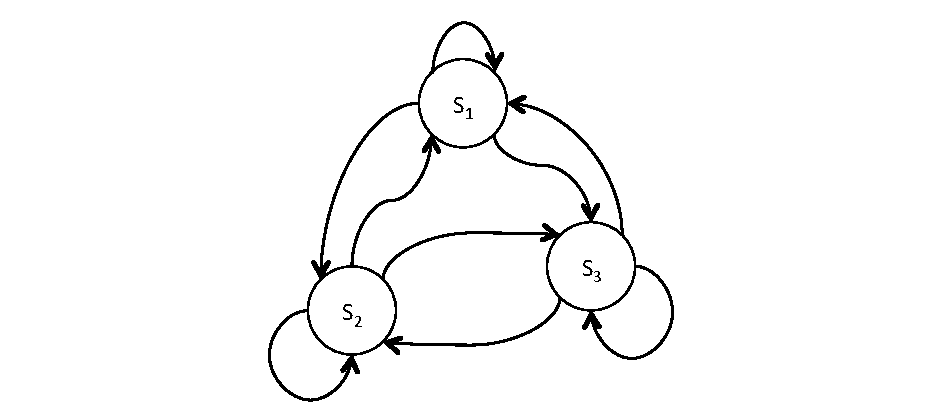
\includegraphics[width=\textwidth]{markov.pdf}
        \caption{State transition process of a Markov chain}
        \label{fig:markov:transition}
        \end{figure}
Illus.\,\ref{fig:markov:transition} visually shows a typical Markov chain.
The state space in this case is finite (three in fact) and 
the process is the transition from the states to one another.

We have given the definition of the state transition matrix 
with Def.\,\ref{defn:markov} in Sec.\,\ref{sec:preliminary:markov:definition}.
For every finite-state time-homogeneous Markov chain, 
we have the following theorem.

		\begin{thm}
		\label{thm:CK}
		For finite-state time-homogeneous Markov chains and any $t,u \in \hn$, we have
			\begin{equation}
			\label{eq:preliminary:markov:CK}
			\bGamma^{(t+u)} = \bGamma^{(t)}\bGamma^{(u)}.
			\end{equation}
		Eq.\,\ref{eq:preliminary:markov:CK} is known as Chapman-Kolmogorov equation.
		\end{thm}
If we denote the $1$-step transition matrix $\bGamma^{(1)}$ as $\bGamma$, 
then we shall deduce the following corollary.
		
		\begin{cor}
		\label{cor:CK}
		For every finite-state time-homogeneous Markov chain and any $t \in \hn$, we have
			\begin{equation}
			\label{eq:preliminary:markov:CK_2}
			\bGamma^{(t)} = \bGamma^t,
			\end{equation}
		that is, the $k$-step transition matrix is entirely decided by the $1$-step transition matrix.
		\end{cor}
Now we give the definition of the initial distribution of a Markov chain,
and we shall find the unconditional distribution of the chain at a given time.

		\begin{defn}
		\label{defn:initial}
		We call the row vector
			\begin{equation}
			\label{eq:preliminary:markov:initial}
			\bdelta(t) = \left(\prob{S_t=1},\dots,\prob{S_t=N}\right)
			\end{equation}
		the unconditional probabilities of a Markov chain at time $t$.
		In particular, we refer to $\bdelta(1) := \bpi$ as the initial distribution of the Markov chain.
		\end{defn}
Then with the definition and Cor.\,\ref{cor:CK}, we have
		\begin{equation}
		\label{eq:preliminary:markov:unconditional}
		\bdelta(t+1) = \bdelta(t)\bGamma = \bpi\bGamma^{t}.
		\end{equation}
The equation implies that the unconditional distribution relies fully on 
the initial distribution and the state transition matrix.


\subsection{Stationary distributions}
\label{sec:preliminary:markov:stationary}
At last we introduce the idea of stationary distribution.

		\begin{defn}
		\label{defn:stationary}
		For a Markov chain, if there exists a row vector $\{v_j \colon j \in \hs\}$ that satisfies
			\begin{subequations}
			\begin{align}
			&v_j  \geq 0, j \in \hs; \\
			&\sum_{j \in \hs} v_j = 1;\\
			&v_j  = \sum_{i \in \hs} v_i\gamma_{ij},
			\end{align}
			\end{subequations}
		then we call $V := \{v_j \colon j \in \hs\}$ the stationary distribution of the Markov chain.
		\end{defn}
The equations above guarantees that $V$ is simutaneously a probability distribution and stationary.

The introduction of stationary distribution is because that 
the state transition matrix will converge.
We state the property as the following theorem.

		\begin{thm}
		\label{thm:stationary}
		For an ergodic finite-space time-homogeneous Markov chain,
		the limit distribution is stationary, i.e.
			\begin{equation}
			\label{eq:preliminary:markov:stationary}
			\lim_{n \ra \infty} \bpi\bGamma^{n} = V.
			\end{equation}
		\end{thm}
One of the results of Thm.\,\ref{thm:stationary} is that forecast result in hidden Markov models
converges with increasing forecast steps
(see Sec.\,\ref{sec:HMM:predeco:forecast}).

%%%%%%%%%%%%%%%%%%%%%%%%%%

\section{K-Means clustering}
\label{sec:preliminary:kmeans}
Data clustering is a popular technique in time series analysis.
It enables us to cluster sub-populations with different properties so that 
more accurate analysis results could be available,
considering the heterogeneity of the sample data.

K-Means, of all existing data clustering techniques,
is the most common and universally acknowledged one.
The name is firstly used in \cite{Macqueen:1967uv}.
The idea originates from signal processing theories, 
which is known as vector quantization (VQ),
and now is prevalent for cluster analysis and data mining.

The standard algorithm for K-Means was proposed by Stuart Lloyd in 1957 and 
by E.\,W.~Forgy in 1965 \cite{Forgy:1965cl} separately, 
which is known as Lloyd-Forgy algorithm.
A more efficient algorithm is proposed by Hartigan in \cite{Hartigan:1975cl}.

Clustering itself has been commonly implemented in financial data analysis
(e.g.\,see \cite{Cont:2001gv,Babu:2012wl,Gupta:2014tp}),
while we introduce the K-Means algorithm merely to find the initial distribution 
of the hidden Markov model (see Sec.\,\ref{sec:system:function:init}),
thus we only provide a very brief introduction here.


\subsection{Model formulation and aims}
\label{sec:preliminary:kmeans:formulation}
Firstly we state the K-Means clustering problem.

Given observation set $\{\bx_1,\bx_2,\dots,\bx_n\}$ where $\bx$ is a $d$-dimensional vector,
we aim to partition the $n$ observations into $k (k\leq n)$ sub-sets $\{S_1,S_2,\dots,S_k\}$
in order to minimize the within-cluster sum of squares (WCSS), 
which is the sum of distance functions of each point in the cluster to the center.
The formulation of this problem is given as follow:
		\begin{equation}
		\label{eq:preliminary:kmeans}
		\min_{\bS} \sum_{i=1}^{k}\sum_{\bx \in S_i} \norm{\bx - \bmu_i}^2,
		\end{equation}
where $\bmu_i$ is the mean of points of $S_i$ (center),
and $\bS$ is the $k$ sub-sets.

The clustering centers found by the K-Means algorithm shall be
appropriate guesses for the initial distribution.


\subsection{The K-Means algorithm}
\label{sec:preliminary:kmeans:algo}
The standard algorithm processes iteratively.

Given a set of initial guess of $k$ means $\{m_1^{(1)},m_2^{(1)},\dots,m_k^{(1)}\}$,
we firstly assign each observation to the cluster whose mean yields the least WCSS,
which is known as the assignment step.
		\begin{equation}
		\label{eq:preliminary:kmeans:assign}
		S_i^{(t)} = \left\{x_p \colon \norm{x_p-m_i^{(t)}}^2 \leq \norm{x_p-m_j^{(t)}}^2,
			\forall j,\ 1\leq j \leq k  \right\}.
		\end{equation}
Each $x_p$ is assigned to one and only one set $S_i$.

Then we calculate the new means to be the centroids of the observations in the new clusters,
which is known as the update step.
		\begin{equation}
		\label{eq:preliminary:kmeans:update}
		m_i^{(t+1)} = \frac{1}{\abs{S_i^{(t)}}} \sum_{x_j \in S_i^{(t)}} x_j.
		\end{equation}
The two steps are performed in sequence until convergence of the result.

Notice that the algorithm only yields a local optimum 
but has no guarantees on finding the global one.
The result is enough for the analysis we will carry out in empirical analysis.
Since the algorithm is not the major concern of this thesis,
the programming realization of K-Means implement 
the \texttt{sklearn.cluster.KMeans} module directly for convenience
(see Appendix \ref{app:code}).


